

\myframe{Lower bound method for OBDD($\land$, reorder)}
{
Let $\Phi=\bigwedge_{i\in I} C_i$ be minimally unsatisfiable CNF
\begin{enumerate}
\item $\Phi'$ is a satisfiable formula associated with $\Phi$. Roughly speaking: $\Phi'$ is $\Phi$ without several clauses.
\begin{itemize}
   \item For $\Phi$=PHP$^{n+1}_{n}$, $\Phi'$=PHP$^{n}_{n}$
   \item For unsatisfiable Tseitin formulas, $\Phi'$ is satisfiable Tseitin formula.
\end{itemize}
\item Prove that any OBDD representation of $\Phi'$ has large size.
\item The last step: $\frac{F_1^{\pi}\land F_2^{\pi}}{0}$. $F_1, F_2$ are satisfiable and $F_1\equiv \bigwedge_{i\in I_1} C_i, F_2\equiv \bigwedge_{i\in I_2} C_i$
and $I_1\neq I_2$, $I_1\cup I_2=I$.
\item Find partial substitution $\rho_1, \rho_2$ with same support: $F_1|_{\rho_1} \land F_2|_{\rho_2}$ is a hard satisfiable formula for OBDD.
Hence either $F_1|_{\rho}^{\pi}$ or $F_2|_{\rho}^{\pi}$ is hard for OBDD, hence $F_1$ or $F_2$ is hard for OBDD.                                                                 
\end{enumerate}
}

\myframe{Lower bounds for OBDD}
{
For particular order $\pi$:
\begin{itemize}
\item $F$, $S=\{x_{\pi(1)}, x_{\pi(2)}, \dots, x_{\pi(\ell)} \}$.
\item Let $\rho_1,\rho_2,\dots, \rho_k$ be partial substitution with support $S$ such that
$F|_{\rho_1}, F|_{\rho_2},\dots,F|_{\rho_k}$ are different functions.
\item Then every $\pi$-OBDD for $F$ has at least $k$ vertices.
\end{itemize}

\pause
For all orders:
\begin{itemize}
\item For arbitrary $S$ that consists of $\ell$ variables.
\end{itemize}

}


\myframe{Pigeonhole principle}
{
\begin{itemize}
\item $PHP^m_n$, $m$ pigeons, $n$ holes.
\item variables $p_{i, j}$, $i \in [m]$, $j \in [n]$;
$p_{i, j}$: $i$-th pigeon is in the $j$-th hole.
\item Clauses:
\begin{itemize}
\item \mycolor{blue}{Long} clauses:
$p_{i, 1} \lor p_{i, 2} \dots \lor p_{i, n}$ for all $i \in [m]$
\item \mycolor{blue}{Short} clauses: $\lnot p_{i, k} \lor \lnot p_{j, k}$ for all $i \neq j
\in [m]$ and all $k \in [n]$.
\end{itemize}
\item $PHP^m_n$ is unsatisfiable iff $m>n$.
\end{itemize}

\pause \mylem Any OBDD for $PHP^n_n$ has size $2^{\Omega(n)}$.

\pause \myth Any OBDD($\land$, reordering)-proof of PHP$^{n+1}_n$ has size $2^{\Omega(n)}$.
}





\myframe{Symbolic quantifier elimination}
{
OBDD($\land, \exists$)-algorithms [Pan, Vardi, 2004] for SAT.

Input: CNF formula $\phi$
\begin{enumerate}
\item Choose order $\pi$, $D^\pi$. Initially $D\equiv 1$.
\item $S:=\{\mbox{clauses of }\phi\}$.
\item While $S\neq \emptyset$ apply the following operations:
\begin{itemize}
\item Conjunction ($\land$)  Choose $C\in S$; $S:=S-C$; $D^{\pi}:=D^{\pi} \land C$
\item Projection ($\exists$) If $x$ does not appear in $S$, then $D^{\pi}:=(\exists x D)^{\pi}$
\end{itemize}
\item If $S=\emptyset$ then report whether $D$ is satisfiable or not.
\end{enumerate}

Running time is polynomially connected with the size of the largest $D$.
}

\myframe{OBDD($\land, \exists$)-algorithms}
{
Upper bounds:
\begin{itemize}
\item{} [Ch{\'{e}}n, Zhang, 2009] Pigeonhole principle PHP$^{n+1}_n$ is easy for OBDD($\land, \exists$)-algorithms.
\item Tseitin formulas are easy for OBDD($\land, \exists$)-algorithms.
\begin{itemize}
\item $\exists x \left\{\begin{aligned} &x+y+z=1 \\ &x+t+f=0 \end{aligned}\right.  \iff y+z+t+f=1$.
\item Sum up all equalities in the connected component.   
\end{itemize}
\end{itemize}                        

Lower bounds:
\begin{itemize}
\item Follows from lower bounds for (tree-like) OBDD($\land$, weakening)-proofs.
\end{itemize}
}

\myframe{OBDD($\land, \exists$, reorder)-algorithms}
{
\begin{itemize}
\item (reorder) Choose $\pi'$ and $F^{\pi'}$ such that $F\equiv D$; $\pi:=\pi'$ and $D:=F$.
\end{itemize}

Our goals:
\begin{itemize}
\item Lower bounds for OBDD($\land, \exists$, reorder)-algorithms
\item Lower bound of type $2^{\Omega(n)}$, where $n$ is number of variables
\item Lower bound for natural formulas.
\end{itemize}

\pause \myth There is a randomized construction of a family of satisfiable formulas $F_n$ on $n$ variables in $O(1)$-CNF such that every
OBDD($\land, \exists, \mbox{ reorder}$)-algorithm runs at least $2^{\Omega(n)}$ steps on $F_n$.
Formula $F_n$ represents a  system of linear equations over $\mathbb{F}_2$
based on checksum matrix of some linear code.
}

\myframe{OBDD size for codes}
{
\begin{itemize}
\item A code $C\subseteq \{0,1\}^n$ recovers $\rho$ fraction of erasures by a list of size $L$
(or $C$ is $(\rho, L)$-erasure list-decodable) if for all $w\in \{0,1,\square\}^n$ with at most $\rho$
fraction of $\square$ there are at most $L$ codewords that are consistent with $w$.
\end{itemize}

\pause
\mylem If $C\subseteq \{0,1\}^n$ is $(\frac{1}{2}+\epsilon, L)$-erasure list-decodable, then any OBDD
for $\chi_C$ has OBDD size at least $\frac{|C|}{L^2}$. Moreover for every $i_1, i_2,\dots, i_k\in [n]$ if $k\le 2\epsilon n$,
then $\exists x_{i_1}\dots \exists x_{i_k} \chi_C$ has OBDD size at least $\frac{|C|}{L^2}$.

\pause \dok
\begin{itemize}
\item Consider some order $\pi$
\item $\exists x_{n-k+1}\dots \exists x_{n} \chi_C(x_1, x_2,\dots, x_n)$
\item We show that there are many substitutions to the first $\frac{n-k}{2}$ variables that produce
different functions.
\pitem $S$ is a set of all $\frac{n-k}{2}$-size prefixes of $C$.
\pitem $L+1$ different codewords can't have same prefixes since $n-\frac{n-k}{2}\le (\frac{1}{2}+\epsilon) n$.
Hence $|S|\ge \frac{|C|}{L}$.
\end{itemize}
}

\myframe{OBDD size for codes}
{
\mylem If $C\subseteq \{0,1\}^n$ is $(\frac{1}{2}+\epsilon, L)$-erasure list-decodable, then any OBDD
for $\chi_C$ has ODBB size at least $\frac{|C|}{L^2}$. Moreover for every $i_1, i_2,\dots, i_k\in [n]$ if $k\le 2\epsilon n$,
then $\exists x_{i_1}\dots \exists x_{i_k} \chi_C$ has OBDD size at least $\frac{|C|}{L^2}$.

\dok (Continue)
\begin{itemize}
%\item Consider some order $\pi$
%\item $\exists x_{n-k+1}\dots \exists x_{n} \chi_C(x_1, x_2,\dots, x_n)$
%\item Consider first $\frac{n-k}{2}$ variables; we show that there are many substitutions to them that produce
%different functions.
\item $S$ is a set of all $\frac{n-k}{2}$-size prefixes of $C$.
%\item $L+1$ different codewords can't have same prefixes since $n-\frac{n-k}{2}\le (\frac{1}{2}+\epsilon) n$.
%Hence
$|S|\ge \frac{|C|}{L}$.
\pitem For every $s\in S$ we define $\rho_s$ that substitutes $x_1\dots x_{(n-k)/2}:=s$.
$\exists x_{n-k+1}\dots \exists x_{n} \chi_C(x_1, x_2,\dots, x_n)|_{\rho_s}$ is satisfiable since $s$
is a prefix of a codeword.
\pitem Let $s_1, s_2,\dots, s_{L+1}$ be different elements of $S$. We claim that
$\rho_{s_i}$ for $i\in [L+1]$ can't produce the same function.
\pitem Let $s_1r$ be a prefix of an element of $C$ of size $n-k$.
\pitem $\exists x_{n-k+1}\dots \exists x_{n} \chi_C(x_1, x_2,\dots, x_n)|_{\rho_{s_1}}(r)=1$, hence
for all $i\in [L+1]$, $s_ir$ is $n-k$ prefix of some element of $C$. Contradiction, since
$\square^{\frac{n-k}{2}}r\square^{k}$ has at most $\frac{1}{2}+\epsilon$ fraction of $\square$.
\pitem Number of different functions $\ge\frac{S}{L}\ge \frac{|C|}{L^2}$.
\end{itemize}           
}

\myframe{Lower bounds for OBDD($\land,\exists$, reorder)-algorithms}
{
\myth Let $A$ be an $0.97 n\times n$ matrix over $\mathbb{F}_2$ such that
\begin{itemize} 
\item  $A$ is a checksum matrix of $(\frac{2}{3}, 10)$-eras. list-decodable code;
\item $A$ contains $t=O(1)$ ones in every row;
\item Every $\frac{n}{12}$ columns of $A$ contain ones in at least $0.96 n$ rows. 
\end{itemize}
Then every
OBDD($\land,\exists$, reorder)-algorithm runs at least $2^{\Omega(n)}$ steps on the formula that encodes $Ax=0$.

\pause \dok
\begin{itemize}
\item Let $D$ be the first diagram  after $\frac{n}{12}$ applications of $\exists$.
\item $D\equiv \exists_1\dots \exists_{n/12} F$, where $F$ is a conjunction of
all clauses from $0.96n$ rows of $A$ and possibly some other clauses.
\end{itemize} \pause
\mylem If $A$ is a checksum matrix of $(\rho, L)$-erasure list-decodable code.
$A'$ is obtained from $A$ by removing of $k$ rows, then $A$ is a checksum matrix of
$(\rho, 2^kL)$-erasure list-decodable code.
\begin{itemize}
\pitem $F$ is char. function of a $(\frac{2}{3}, 2^{0.1 n} 100)$-erasure list-decodable code of size at least
$|C|$. Hence $|D|\ge 2^{\Omega(n)}$.
\end{itemize}
}

\myframe{Construction of code}
{
\mylem [Guruswami, 2003] If $C$ is a code with relative distance $\delta$, then for every $\epsilon > 0$ the code $C$ is $((2 - \epsilon) \delta,
    \frac{2}{\epsilon})$-erasure list-decodable.

\pause{}
[Gallager, 1962]

$B=\left( \underbrace{\fbox{$I_{n/t}$} \fbox{$I_{n/t}$}\dots \fbox{$I_{n/t}$}}_{t\mbox{ times}}\right)$
is $n/t \times n$ matrix with $t$ ones per row.
$A=
    \left(
        \begin{array}{c}
            {[}\mbox{ 1st random perm. of columns of }B {]}\\
            {[}\mbox{2nd random  perm. of columns of }B {]}\\
            \vdots \\
            {[}\mbox{$r$-th random perm. of columns of }B {]}
        \end{array}
    \right)
$ is $\frac{rn}{t}\times n$ matrix with $t$ ones per row.

\mylem $\exists t$ such that for $r=0.97 t$ w.h.p $A$ defines a code with relative distance
$0.49$. W.h.p every $\frac{n}{12}$ columns of $A$ intersects at least $0.96n$ rows.

}

\myframe{Open problems}
{
\begin{enumerate}
\item Lower bound for OBDD$(\land, \mbox{ weakening, reorder})$-proofs;
%\item Separate OBDD$(\land, \mbox{ weakening})$ and OBDD$(\land, \mbox{ weakening, reorder})$-proofs;
\item Does OBDD$(\land, \mbox{ weakening})$ simulate OBDD$(\land, \mbox{ reorder})$?
\item Is it possible to simulate OBDD($\land$)-proofs by OBDD($\land, \exists$)-algorithms?
\item Prove lower bound for OBDD($\land, \exists$,\mbox{ reorder})-algorithms on unsatisfiable linear systems.
\item Compare OBDD($\land$)-proofs with constant degree Frege.
\end{enumerate}
}

%\end{document}

\myframe{Tseitin formulas}
{
\begin{itemize}
\item $G(V,E)$ is undirected constant-degree graph;
\item For every $e\in E$: $x_e$ Boolean variable;
\item $c:V\to \{0,1\}$ labelling function
\item $TS_{G,c}=\bigwedge_{v\in v} \left( \bigoplus_{u: (u,v)\in E} x_{(u,v)} = c(v)\right)$
\end{itemize}

\mylem $TS_{G,c}$ is satisfiable iff for every connected component $U$, $\bigoplus_{v\in U} c(v)=0$.
}

\myframe{OBDD for satisfiable Tseitin formula}
{

\begin{itemize}
\item Let $TS_{G,c}$ be satisfiable Tseitin formula.
\item Consider some order $\pi$;
\item Let $S$ be a set that consists first $\ell$ edges according $\pi$
\item Consider some substitution $\rho$ with support $S$.
\item $TS_{G,c}|_\rho=TS_{G',c+f}$, where $G'(V, E\setminus S)$ and $f:V\to \{0,1\}$ is a modification of labels made by $\rho$.
\item Different functions: different $f$ and $TS_{G',c+f}$ is satisfiable.
\item We estimate the number of $f$ such that
\begin{itemize}
\item $TS_{G',c+f}$ is satisfiable
\item $f$ can be obtained by a substitution \pause $\iff$ $TS_{G'',f}$ is satisfiable, where $G''(V, S)$.
\end{itemize}
\item  $\sharp G'+\sharp G''$ linear conditions on $f$.
\item Hence number of different functions at least $2^{n-\sharp G'-\sharp G''}$
\end{itemize}
}

\myframe{Tseitin formulas on expanders}
{
\myth If $G(V,E)$ is good enough expander with $|V|=n$ then  $\exists \ell$:
$\forall S\subseteq E$ if $|S|=\ell$ then $\sharp G'(V, E\setminus S)+ \sharp G''(V,S)\le (1-\epsilon) n$.

\pause \mycor Every OBDD representation of satisfiable $TS_{G,c}$ has size at least $2^{\Omega(n)}$.

\pause \mycor If $G$ differs from good enough expander by at most $o(n)$ edges, then
OBDD representation of satisfiable $TS_{G,c}$ has size at least $2^{\Omega(n)}$.

\pause \mylem Good enough expander is connected and remains connected after deleting of any two vertices
and edges from the shortest path between them.

}

\myframe{Lower bound for unsatisfiable Tseitin formula}
{
\myth If $G(V,E)$ is good enough expander with $|V|=n$ and $TS_{G,c}$ is unsatisfiable then the size of any OBDD($\land$, reorder)-proof
of $TS_{G,c}$ is at least $2^\Omega(n)$.

\dok

\parbox{.45\textwidth}{
\begin{itemize}
\item The last step: $\frac{F_1^{\pi}\land F_2^{\pi}}{0}$. $F_1, F_2$ are satisfiable.
%$F_1$ and $F_2$ are conjunction of some (but not all)
%clauses of $TS_{G,c}$. Every clause is either in $F_1$ or $F_2$.
\item Let $F_1$ does not contains $C_u$ and $F_2$ does not contain $C_v$ and $(u,v)\notin E$
\item Let $P$ be the shortest $uv$-path
\end{itemize}
}
\parbox{.45\textwidth}{
\begin{figure}[ht]
\begin{center}
  \scalebox{0.35}{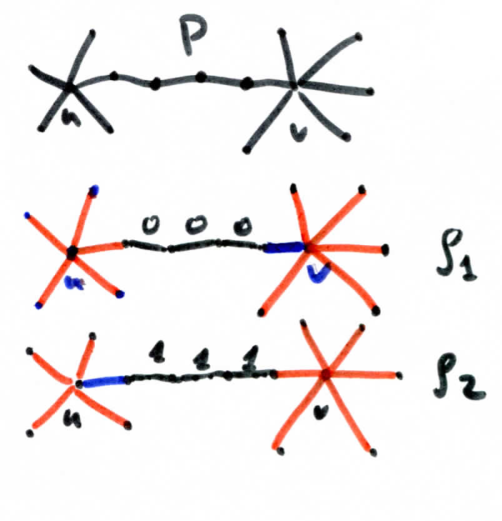
\includegraphics{pics/tseitin.pdf}}
\end{center}
 $F_1|_{\rho_1} \land F_2|_{\rho_2}$ is almost satisfiable $TS_{\tilde G, c'}$, where $\tilde G(V\setminus\{u,v\},E\setminus P)$.
%Hence $F_1|_{\rho_1} \land F_2|_{\rho_2}$ has large OBDD.

\end{figure}
}                     


}
